% !TeX spellcheck = sk_SK-Slovak
\chapter{Vstupné dáta a ich štruktúra}

\label{kap:strukSpravy} % id kapitoly pre prikaz ref

Táto kapitola sa zameriava na pochopenie vstupných dát a približnú lokalizáciu hľadaných informácii v nich.

\section{Zdroj dát}

Prepúšťacie správy a krvné výsledky ktoré náš systém spracováva sú správami pacientov ktorí boli v období od marca roku 2020 do decembra roku 2021 hospitalizovaní na klinike infektológie a geografickej medicíny univerzitnej nemocnice v Bratislave.

\section{Výzor vstupných dát}

Vstupné dáta z ktorých sa náš systém snažíme získať informácie o pacientovi sú v tvare textu obsahujúceho prepúšťaciu správu a krvné výsledky. Väčšina textu v prepúšťacej správe nie je generovaná automaticky nemocničným informačným systémom ale je písaná lekárom čo spôsobuje, že každá správa je do určitej miery originálna.

Napriek tomu existuje základná štruktúra ktorú majú spoločnú takmer všetky prepúšťacie správy vďaka ktorej je možné túto správu rozdeliť do blokov (viď obrázok \ref{obr:sprava}) ktoré obsahujú špecifické informácie. Teraz si prejdeme, čo obsahujú jednotlivé bloky a čo z nich sa my snažíme získať.

\begin{figure}
	%vlozenie samotneho obrazku vycentrovaneho a vhodnej velkosti
	%obrazok je v subore images/cervik.png
	\centerline{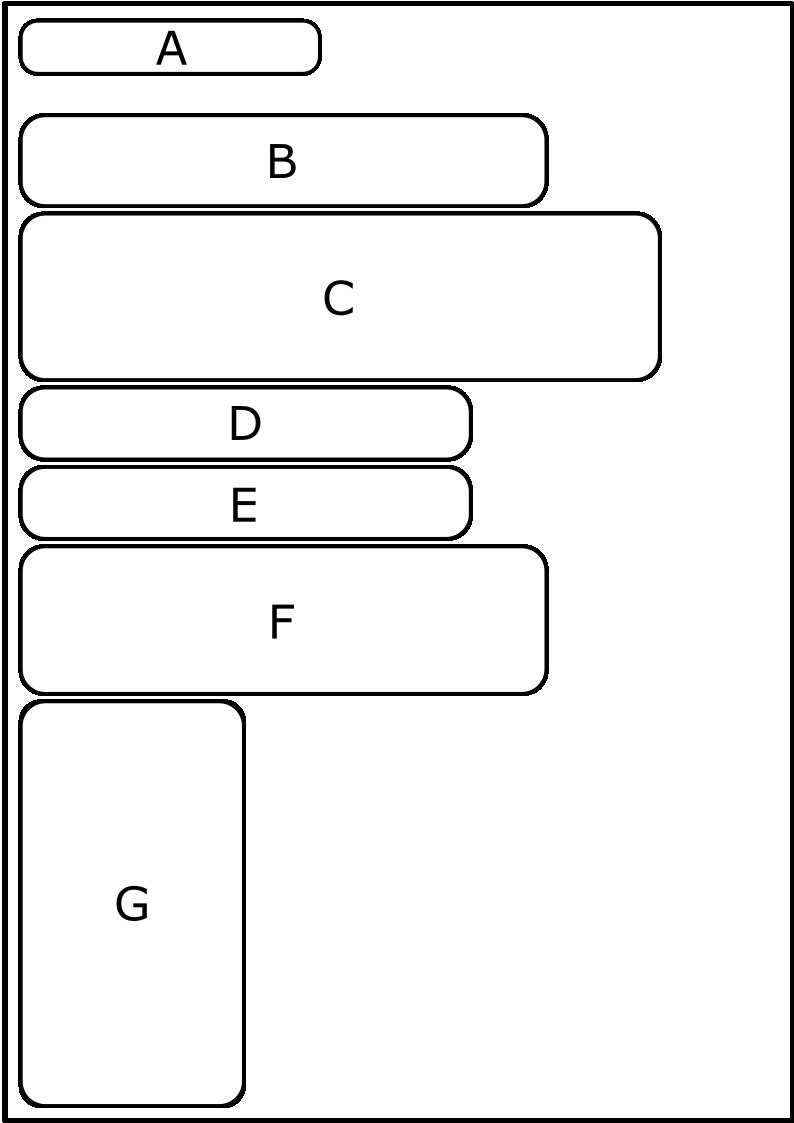
\includegraphics[width=0.4\textwidth]{images/vyzor_spravy}}
	%popis obrazku
	\caption[Rozloženie správy]{Rozdelenie správy do špecifických blokov podľa ich obsahu}
	%id obrazku, pomocou ktoreho sa budeme na obrazok odvolavat
	\label{obr:sprava}
\end{figure}

\subsection{Blok A - Osobné údaje a obdobie hospitalizácie}
\label{blokA}
Bloku A je dvojriadková hlavička v ktorej sa nachádzajú základné osobné údaje pacienta, čiže jeho celé meno a rodné číslo. Zároveň sa tam nachádza dátum priatia a dátum prepustenia daného pacienta. Všetky tieto informácie sa snažíme získať.

\subsection{Blok B - Anamnéza}
\label{blokB}
Tento blok obsahuje anamnézu pacienta, čiže súhrn informácii o zdravotnom stave pacienta v minulosti a pri prijatí do nemocnice. Z informácii o minulosti pacienta nás zaujíma informácia o dlhodobých alebo prekonaných chorobách a problémoch ako sú cukrovka, astma, demencia, infarkt myokardu, artériová hypertenzia, fibrilácia predsiení, srdcové zlyhanie a ďalšie. Z informácii o stave pacienta pri priatí získavame informáciu o výške, váhe a saturácii krvi kyslíkom.

\subsection{Blok C - Vyšetrenia}
\label{blokC}
Blok C obsahuje informácie o vykonaných vyšetreniach, pre nás sú podstatné výsledky testov na protilátky proti vírusu SARS-CoV-2 typu IgG a IgM pri prijatí, prípadne výsledok testu na ochorenie CDI (Infekcia spôsobená Clostridium difficile) známe aj ako kolitída.

Zároveň sa tu nachádzajú aj výsledky krvných testov avšak tie sa tu nemusia nachádzať úplné. Preto ich náš systém považuje iba za kontrolné a samotné informácie o krvných výsledkoch sa získavajú z posledného bloku (\ref{blokG}).

\subsection{Blok D - Terapia}
\label{blokD}
V tomto bloku sú informácie o terapii, čiže o liečbe ktorá bola pacientovi počas hospitalizácie podaná. Odtiaľto získavame informáciu o liekoch ktoré pacient počas hospitalizácie užíval a o tom či bola pacientovi podaná oxygenoterapia a v prípade, že áno aj o aký typ oxygenoterapie išlo.

\subsection{Blok E - Epikríza}
\label{blokE}
Tento blok obsahuje časť správy s názvom epikríza čiže záverečná, súhrnná správa o pacientovi a o priebehu jeho choroby a hospitalizácie. Jedinou získavanou informáciou je informácie o tom či počas hospitalizácie pacient umrel. 

Táto časť sa dá zároveň využiť aj na prípadnú kontrolu iných získavaných informácii keďže môže obsahovať informáciu o iných ochoreniach pacienta, jeho liečbe, prípadne o prítomnosti protilátok proti vírusu SARS-CoV-2 či typu oxygenoterapie.

\subsection{Blok F - Záver, odporúčania, špecifické nálezy}

Blok F obsahuje zvyšné časti správy ako sú záver, odporúčania a špecifické nálezy. Obsah tohto bloku je výrazne nekonzistentný a jeho jednotlivé časti nemusia byť vôbec prítomné v správe. Našťastie pre nás tento blok neobsahuje žiadne získavané informácie.

\subsection{Blok G - Krvné výsledky}
\label{blokG}
Záverečný blok už nie je priamo prepúšťacia správa ale ide o krvné výsledky pacienta ktoré narozdiel od výsledkov v bloku C (\ref{blokC}) sa tu nachádzajú úplné. Každý testovaný parameter je v samostatnom riadku v tvare ''[názov]: [hodnota]''.

\section{Problémy pri rozdelení dát na bloky} 

Pri snahe o implementáciu tohto delenia sme zistili, že aj napriek tomu, že sa pomerne veľký počet správ dal do takýchto blokov rozdeliť, tak sa objavilo niekoľko problémov či už pri samotnom delení správy alebo pri informačnom obsahu jednotlivých blokov kvôli ktorým sa ukazuje vhodnejšie takéto riešenie vôbec nepoužiť alebo použiť nejakú robustnejšiu verziu tohto delenie. Niektoré z nájdených problémov si teraz opíšeme.

\subsection{Problém nenájdených blokov}

Pri kontrole správ rozdelených do blokov sme zistili, že sa občas stávalo, že náš softvér nebol schopný nájsť niektorý z blokov, väčšinu z týchto problémov vieme rozdeliť do troch skupín: chýbajúci alebo nesprávne ohraničený blok F, blok E skrytý v bloku F, chýbajúci alebo nesprávne napísaný začiatok bloku.

Prvý problém pre nás nepredstavuje veľký problém keďže v bloku F by sa nemali nenachádzajú hľadané informácie. 

Druhý problém je o niečo horší keďže blok E je pre nás dôležitý ale tento problém bolo jednoduché opraviť tým, že ak softvér nenájde blok E pri prvotnom delení správy ešte skontroluje či sa v bloku F náhodnou nenachádza, respektíve informácie získavané z bloku E bude hľadať v bloku F.

Tretí problém je najproblematickejší. Správne určenie začiatku a konca bloku sa ukázalo komplikovanejšie ako sme očakávali. Ak softvér nenájde kľúčové slová ktorými sa vo väčšine prípadov jednotlivé bloky začínajú či už z dôvodu absencie týchto slov ale neočakávanej chyby v týchto slovách, tak nie je schopný určiť začiatok bloku s dostatočnou presnosťou. Preto sa stávalo, že softvér niektoré bloky nenašiel a lebo ich pripojil k iným blokom. Tento problém sa stal jedným z hlavných dôvodov zmeny prístupu k predspracovaniu dát.

\subsection{Problém nesprávne umiestnených dát}

Ako ďalší veľký problém sa ukazuje to, že niektoré informácie sa nenachádzajú na očakávanom mieste. Zväčša išlo o informácie o anamnéze pacienta a výsledkoch jeho vyšetrení ktoré sme predpokladali, že nájdeme v blokoch B, respektíve C avšak časť týchto informácii sa nachádzala až v bloku F.

Tento problém samotný sa dá riešiť tým, že informácie ktoré hľadáme v blokoch B a C budeme hľadať aj v bloku F. Avšak tento problém spôsobuje, že problém ktorý máme s nájdením a správnym ohraničením bloku F sa stáva relevantným a treba ho riešiť, nanešťastie tento problém je podobný problému ohraničeniu ostatných blokov a preto je jeho riešenie pomerne komplikované.

\section{Riešenia problémov s rozdelením dát do blokov}

Skúšaním rôznych spôsobov riešenia problémov ktoré sa vyskytli pri našom pôvodnom delení sa ukázalo, že nie je vhodné sa snažiť riešiť prípady nesprávneho rozdelenia textu do pôvodných blokov ale zmenšiť počet blokov tak aby sme mali istotu, že ich systém bude schopný správne identifikovať. Konkrétne s takýmto prístupom vyskúšali dve riešenia.

\subsection{Homogénny text}

Jednou možnosťou je považovať celý text ako jeden homogénny text v ktorom hľadáme všetky informácie. V tomto prípade nedochádza k deleniu textu vďaka čomu nemôžu vzniknúť spomínané problémy. 

Problémom tohto prístupu je, že zbytočne hľadá niektoré informácie aj na miestach kde vieme, že sa nikdy nebudú nachádzať čo ho spomaľuje. Zároveň v prípade krvných výsledkov je pre systém zložité rozlíšiť, či nájdený výsledok by patril do pôvodného bloku C alebo G čo môže viesť k získaniu nesprávnych hodnôt.

\subsection{Menej väčších blokov}
\label{spravaLepsie}

Druhý prístup využíva rozdelenie do blokov rovnako ako pôvodný prístup, ale namiesto 7 blokov má toto nové rozdelenie iba 3 bloky, vďaka čomu nemusíme hľadať všetky informácie v celom texte a zároveň je systém schopný veľmi presne určiť začiatky jednotlivých blokov. 

Výzor nového rozdelenia môžeme vidieť na obrázku \ref{obr:sprava_uprava}. Vidíme, že jediná zmena ktorá nastala je taká, že sme bloky B až F spojili do jedného bloku s názvom B a pôvodný blok G sme premenovali na blok C. 

Toto rozdelenie rieši všetky vyššie spomenuté problémy vďaka tomu, že o bloku A vieme, že vždy bude mať tvar dvojriadkovej hlavičky čo sa nám pri vytváraní a testovaní systému potvrdilo. Podobne pôvodný blok G čiže nový blok C nie je súčasťou samotnej prepúšťacej správy ale sú to krvné výsledky pacienta ktoré sú v našom vstupe vždy až za správou a majú tvar dvojíc testovaný parameter a výsledok testu vďaka čomu je jednoduché ich oddeliť od textu správy. V prípade nového bloku B sa ukazuje, že jeho ďalšie delenie vytvára vyššie spomenuté problémy preto ho nechávame pohromade.

\begin{figure}
	%vlozenie samotneho obrazku vycentrovaneho a vhodnej velkosti
	%obrazok je v subore images/cervik.png
	\centerline{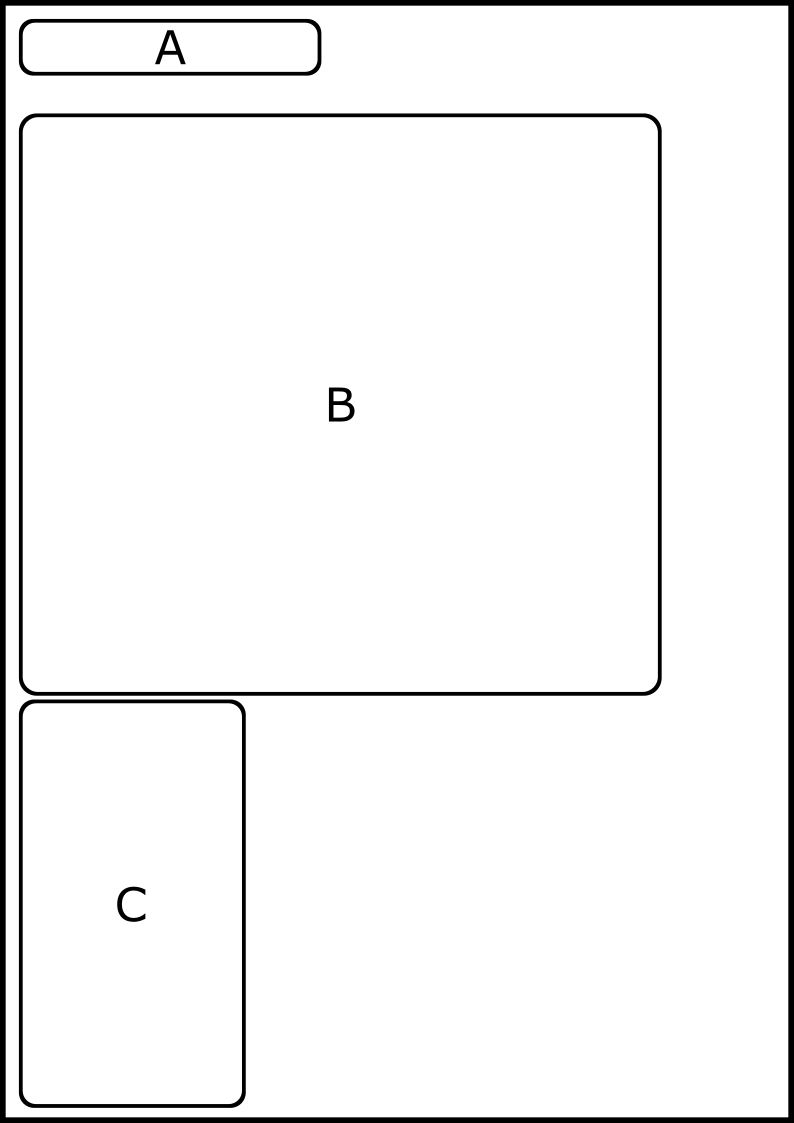
\includegraphics[width=0.4\textwidth]{images/vyzor_spravy_vylepsena}}
	%popis obrazku
	\caption[Upravené rozloženie správy]{Upravené rozdelenie správy do menšieho počtu väčších blokov}
	%id obrazku, pomocou ktoreho sa budeme na obrazok odvolavat
	\label{obr:sprava_uprava}
\end{figure}
   
\section{Predspracované dáta}
\label{predSprac}
Okrem vstupných dátach o pacientoch sme na účely kontroly či náš systém funguje správne dostali v dispozícii aj niekoľko desiatok predspracovaných pacientov, čiže pacientov u ktorých sme mali ich prepúšťaciu správu a krvné výsledky a zároveň sme poznali získavané informácie. 

Problémom týchto dát však bolo, že často boli pre konkrétneho pacienta buď nekompletné alebo obsahovali informáciu ktorá sa nenachádzala ani v správe, ani v krvných výsledkoch alebo boli nesprávne čo bolo spôsobené tým, že tieto dáta boli získavané iným spôsobom. Tieto dáta boli získavané tak, že poverená osoba dostala prístup do nemocničného informačného systému z ktorého následne ručne jednotlivé dáta získavala. Konkrétne problém chýbajúcich dát boli často spôsobený tým, že v čase spracovávania pacienta daný pacient ešte nebol prepustený z nemocnice, v prípade problému dát nenachádzajúcich sa v prepúšťacej správe a krvných výsledkov išlo o prípady kedy lekár túto informáciu do prepúšťacej správy nedal ale v systéme sa nachádzala a v prípade nesprávnych údajov išlo s zväčša o ľudskú chybu keďže tieto dáta boli získavané ručne.

